\documentclass{beamer}

\mode<presentation>
{
    \usetheme{rwth}
    \setbeamercovered{transparent = 28}
}

\usepackage{graphicx}
\usepackage{subfigure}
\usepackage[utf8]{inputenc}
%\usepackage{enumitem}
\usepackage{hyperref}
\usepackage{listings}
%\setlist[description]{leftmargin=0.25cm,labelindent=0.25cm}

\usepackage{array}
\setlength\extrarowheight{2pt}

\usepackage{subfigure}
\usepackage{tikz}
\usepackage{pgfplots}
\usetikzlibrary{arrows.new}
\usetikzlibrary{fadings}

\title{Understanding Convolutional Neural Networks}
\author{David Stutz}
\date{July 24th, 2014}

\RWTHtoc{Table of Contents}
\begin{document}
	\nocite{*}
	\RWTHtitle
	
	\section*{Table of Contents}
	\begin{frame}{Table of Contents}
 		\tableofcontents
	\end{frame}
	
	\section{Motivation}
	\begin{frame}{Motivation}
		Convolutional networks represent specialized networks for application in computer vision:
		\vskip .25em
		
		\begin{itemize}
			\item they accept images as raw input (preserving spatial information),
			\item and build up (learn) a hierarchy of features (no hand-crafted features necessary).
		\end{itemize}
		\vskip 1em
		
		\pause
		
		Problem: Internal workings of convolutional networks not well understood~...
		\vskip .25em
		
		\begin{itemize}
			\item Unsatisfactory state for evaluation and research!
		\end{itemize}
		\vskip 1em
		
		Idea: Visualize feature activations within the network ...
	\end{frame}
	
%	\begin{frame}{Motivation -- Questions}
%		Questions answered in this talk:
%		\vskip 1em
%		
%		\begin{itemize}
%			\item What are neural networks?
%		\end{itemize}
%	\end{frame}
	
	\section{Neural Networks and Network Training}
	\subsection{Multilayer Perceptrons}
	\begin{frame}{Multilayer Perceptrons}		
		A multilayer perceptron represents an adaptable model $y(\cdot, w)$ able to map $D$-dimensional input to $C$-dimensional output:
		\begin{align}
			y(\cdot, w) : \mathbb{R}^D \rightarrow \mathbb{R}^C, x \mapsto y(x,w) = 
			\begin{pmatrix}
				y_1(x,w)\\
				\vdots\\
				y_C(x,w)\\
			\end{pmatrix}.
		\end{align}
		\vskip 1em
		
		In general, a $(L + 1)$-layer perceptron consists of $(L + 1)$ layers, each layer $l$ computing linear combinations of the previous layer $(l - 1)$ (or the input).
	\end{frame}
	
	\begin{frame}{Multilayer Perceptrons -- First Layer}		
		On input $x \in \mathbb{R}^D$, layer $l = 1$ computes a vector $y^{(1)} := (y_1^{(1)}, \ldots, y_{m^{(1)}} ^{(1)})$ where
		\begin{align}
			\label{eq:layer-one}
			y_i^{(1)} = f\left(z_i^{(1)}\right) \quad \text{ with } z_i^{(1)} = \sum_{j = 1} ^D w_{i,j}^{(1)} x_j + w_{i,0}^{(1)}.
			\begin{tikzpicture}[overlay,remember picture]
    				\draw[-latex new,arrow head=0.25cm,RWTHblue,shorten >=3pt,shorten <=3pt,thick,out=180,in=285] (-4,-1) node{$i^{\text{th}}$ component is called ``unit $i$''} (-6.5,-1) to (-7.5,-0.1);
    				%\draw[-latex new,arrow head=0.25cm,RWTHblue,shorten >=3pt,shorten <=3pt,thick,out=180,in=90] (-7,1) node{layer $l = 1$} (-8,1) to (-9.25,0.4);
  			\end{tikzpicture}
		\end{align}
		\vskip 1em
		where $f$ is called activation function and $w_{i,j}^{(1)}$ are adjustable weights.
	\end{frame}
	
	\begin{frame}{Multilayer Perceptrons -- First Layer}
		What does this mean?
		\vskip 1em
		Layer $l = 1$ computes linear combinations of the input and applies an (non-linear) activation function ...
		\vskip 1em
		
		The first layer can be interpreted as generalized linear model:
		\begin{align}
			y_i^{(1)} = f\left(\left(w_i^{(1)}\right)^Tx + w_{i,0}^{(1)}\right).
		\end{align}
		\vskip 1em
		
		Idea: Recursively apply $L$ additional layers on the output $y^{(1)}$ of the first layer.
	\end{frame}

	\begin{frame}{Multilayer Perceptrons -- Further Layers}
		In general, layer $l$ computes a vector $y^{(l)} := (y_1^{(l)}, \ldots, y_{m^{(l)}}^{(l)})$ as follows:
		\begin{align}
			y_i^{(l)} = f\left(z_i^{(l)}\right) \quad \text{ with } z_i^{(l)} = \sum_{j = 1} ^{m^{(l-1)}} w_{i,j}^{(l)} y_j^{(l - 1)} +w_{i,0}^{(l)}.
		\end{align}
		\vskip 1em
		
		Thus, layer $l$ computes linear combinations of layer $(l - 1)$ and applies an activation function ...
		\vskip 1em
	\end{frame}
	
	\begin{frame}{Multilayer Perceptrons -- Output Layer}
		Layer $(L + 1)$ is called output layer because it computes the output of the multilayer perceptron:
		\begin{align}
			y(x,w) = 
			\begin{pmatrix}
				y_1(x,w)\\
				\vdots\\
				y_C(x,w)\\
			\end{pmatrix} := 
			\begin{pmatrix}
				y_1^{(L + 1)}\\
				\vdots\\
				y_C^{(L + 1)}\\
			\end{pmatrix} = 
			y^{(L+1)}
		\end{align}
		where $C = m^{(L + 1)}$ is the number of output dimensions.
	\end{frame}

	\begin{frame}{Network Graph}
		\begin{figure}[t]
			\centering
			\begin{tikzpicture}[shorten >=1pt]
				\tikzstyle{unit}=[draw,shape=circle,minimum size=1.15cm]
				%\tikzstyle{hidden}=[draw,shape=circle,fill=black!25,minimum size=1.15cm]
				\tikzstyle{hidden}=[draw,shape=circle,minimum size=1.15cm]

				\node[unit](x0) at (-0.5,3.5){$x_1$};
				\node[unit](x1) at (-0.5,2){$x_2$};
				\node at (-0.5,1){\vdots};
				\node[unit](xd) at (-0.5,0){$x_D$};

				\node[hidden](h10) at (2.5,4){$y_1^{(1)}$};
				\node[hidden](h11) at (2.5,2.5){$y_2^{(1)}$};
				\node at (2.5,1.5){\vdots};
				\node[hidden](h1m) at (2.5,-0.5){$y_{m^{(1)}}^{(1)}$};

				\node(h22) at (4.25,1){};
				\node(h21) at (4.25,3){};
		
				\node(d2) at (4.5,1){$\ldots$};
				\node(d1) at (4.5,3){$\ldots$};

				\node(hL12) at (4.75,1){};
				\node(hL11) at (4.75,3){};

				\node[hidden](hL0) at (6.5,4){$y_1^{(L)}$};
				\node[hidden](hL1) at (6.5,2.5){$y_2^{(L)}$};
				\node at (6.5,1.5){\vdots};
				\node[hidden](hLm) at (6.5,-0.5){$y_{m^{(L)}}^{(L)}$};

				\node[unit](y1) at (9.5,3.75){$y_1^{(L+1)}$};
				\node[unit](y2) at (9.5,2){$y_2^{(L+1)}$};
				\node at (9.5,1){\vdots};	
				\node[unit](yc) at (9.5,-0.25){$y_C^{(L+1)}$};

				\draw[-latex new,arrow head=0.15cm] (x0) -- (h10);
				\draw[-latex new,arrow head=0.15cm] (x0) -- (h11);
				\draw[-latex new,arrow head=0.15cm] (x0) -- (h1m);

				\draw[-latex new,arrow head=0.15cm] (x1) -- (h10);
				\draw[-latex new,arrow head=0.15cm] (x1) -- (h11);
				\draw[-latex new,arrow head=0.15cm] (x1) -- (h1m);

				\draw[-latex new,arrow head=0.15cm] (xd) -- (h10);
				\draw[-latex new,arrow head=0.15cm] (xd) -- (h11);
				\draw[-latex new,arrow head=0.15cm] (xd) -- (h1m);

				\draw[-latex new,arrow head=0.15cm] (hL0) -- (y1);
				\draw[-latex new,arrow head=0.15cm] (hL0) -- (yc);
				\draw[-latex new,arrow head=0.15cm] (hL0) -- (y2);

				\draw[-latex new,arrow head=0.15cm] (hL1) -- (y1);
				\draw[-latex new,arrow head=0.15cm] (hL1) -- (yc);
				\draw[-latex new,arrow head=0.15cm] (hL1) -- (y2);

				\draw[-latex new,arrow head=0.15cm] (hLm) -- (y1);
				\draw[-latex new,arrow head=0.15cm] (hLm) -- (y2);
				\draw[-latex new,arrow head=0.15cm] (hLm) -- (yc);

				\draw[-latex new,arrow head=0.15cm,path fading=east] (h10) -- (h21);
				\draw[-latex new,arrow head=0.15cm,path fading=east] (h10) -- (h22);
		
				\draw[-latex new,arrow head=0.15cm,path fading=east] (h11) -- (h21);
				\draw[-latex new,arrow head=0.15cm,path fading=east] (h11) -- (h22);
		
				\draw[-latex new,arrow head=0.15cm,path fading=east] (h1m) -- (h21);
				\draw[-latex new,arrow head=0.15cm,path fading=east] (h1m) -- (h22);
		
				\draw[-latex new,arrow head=0.15cm,path fading=west] (hL11) -- (hL0);
				\draw[-latex new,arrow head=0.15cm,path fading=west] (hL12) -- (hL0);
		
				\draw[-latex new,arrow head=0.15cm,path fading=west] (hL11) -- (hL1);
				\draw[-latex new,arrow head=0.15cm,path fading=west] (hL12) -- (hL1);
		
				\draw[-latex new,arrow head=0.15cm,path fading=west] (hL11) -- (hLm);
				\draw[-latex new,arrow head=0.15cm,path fading=west] (hL12) -- (hLm);
		
				\draw [decorate,decoration={brace,amplitude=10pt},xshift=-4pt,yshift=0pt] (-1,4) -- (0.25,4) node [black,midway,yshift=+0.6cm]{input};
				\draw [decorate,decoration={brace,amplitude=10pt},xshift=-4pt,yshift=0pt] (2,4.5) -- (3.25,4.5) node [black,midway,yshift=+0.6cm]{$1^{\text{st}}$ layer};
				\draw [decorate,decoration={brace,amplitude=10pt},xshift=-4pt,yshift=0pt] (6,4.5) -- (7.25,4.5) node [black,midway,yshift=+0.6cm]{$L^{\text{th}}$ layer};
				\draw [decorate,decoration={brace,amplitude=10pt},xshift=-4pt,yshift=0pt] (9,4.5) -- (10.25,4.5) node [black,midway,yshift=+0.6cm]{output};
			\end{tikzpicture}
			\label{fig:multilayer-perceptron}
		\end{figure}
	\end{frame}
	
	\begin{frame}{Activation Functions -- Notions}
		How to choose the activation function $f$ in each layer?
		\vskip .25em
		
		\begin{itemize}
			\item Non-linear activation functions will increase the expressive power: Multilayer perceptrons with $L + 1 \geq 2$ are universal approximators~\cite{HornikStinchcombeWhite:1989}!
			
			\pause
			
			\item Depending on the application: For classification we may want to interpret the output as posterior probabilities:
			\begin{align}
				y_i(x,w) \overset{!}{=} p(c = i|x)
			\end{align}
			where $c$ denotes the random variable for the class.
		\end{itemize}
	\end{frame}
	
	\begin{frame}{Activation Functions}
		Usually the activation function is chosen to be the logistic sigmoid:
		\vskip 1em
		\begin{minipage}{0.45\textwidth}
			\begin{align}
				\sigma (z) = \frac{1}{1 + \exp(-z)}\notag
			\end{align}
		\end{minipage}
		\begin{minipage}{0.45\textwidth}
    			\begin{tikzpicture}[scale=1,baseline]
				\begin{axis}[tick label style={font=\scriptsize},label style={font=\small},width=5cm,height=5cm,ylabel=$\sigma(z)$,ylabel style={yshift=-0.25cm},xlabel=$z$,ymin=0,xlabel style={yshift=-0.0cm},ymax=1,xmin=-4,xmax=4,axis lines=left,ytick={0,1},xtick={-2,0,2}]
					\addplot[RWTHblue,smooth,thick] {1/(1+exp(-x))};
				\end{axis}
			\end{tikzpicture}
		\end{minipage}
		\vskip 0.5em
		which is non-linear, monotonic and differentiable.
	\end{frame}
	
	\begin{frame}{Activation Functions}
		Alternatively, the hyperbolic tangent is used frequently:
		\begin{align}
			\tanh(z).
		\end{align}
		\vskip 1em
		
		\pause
		
		For classification with $C > 1$ classes, layer $(L + 1)$ uses the softmax activation function:
		\begin{align}
			y_i^{(L+1)} = \sigma(z^{(L + 1)},i) = \frac{\exp(z_i^{(L + 1)})}{\sum_{k = 1}^C \exp(z_k^{(L + 1)})}.
		\end{align}
		\vskip 1em
		
		Then, the output can be interpreted as posterior probabilities.
	\end{frame}
	
	\subsection{Network Training}
	\begin{frame}{Network Training -- Notions}
		By now, we have a general model $y(\cdot, w)$ depending on $W$ weights.
		\vskip 1em
		
		Idea: Learn the weights to perform
		\vskip .25em
		
		\begin{itemize}
			\item regression,
			\item or classification.
		\end{itemize}
		\vskip 1em
		
		We focus on classification.
	\end{frame}
	
	\begin{frame}{Network Training -- Training Set}
		Given a training set
		\begin{align}
			U_S = \{(x_n, t_n) : 1 \leq n \leq N\},
			\begin{tikzpicture}[overlay,remember picture]
    				\draw[-latex new,arrow head=0.25cm,RWTHblue,shorten >=3pt,shorten <=3pt,thick,out=180,in=90] (0.5,1.25) node{\begin{tabular}{l}$C$ classes:\\$1$-of-$C$ coding scheme\end{tabular}} (-1.5,1.25) to (-2.8,0.3);
  			\end{tikzpicture}
		\end{align}
		learn the mapping represented by $U_S$ ...
		\vskip 1em
		
		\pause
		
		by minimizing the squared error
		\begin{align}
			E(w) = \sum_{n = 1}^N E_n(w) = \sum_{n = 1}^N \sum_{i = 1}^C \left(y_i(x_n,w) - t_{n,i}\right)^2
		\end{align}
		using iterative optimization.
	\end{frame}
	
	\begin{frame}{Training Protocols}
		We distinguish ...
		\vskip .25em
		
		\begin{description}
			\item[Stochastic Training] A training sample $(x_n, t_n)$ is chosen at random, and the weights $w$ are updated to minimize $E_n(w)$.
			\vskip 1em
			
			\pause
			
			\item[Batch and Mini-Batch Training] A set $M \subseteq \{1,\ldots,N\}$ of training samples is chosen and the weights $w$ are updated based on the cumulative error $E_M(w) = \sum_{n \in M} E_n(w)$.
		\end{description}
		\vskip 1em
		
		\pause
		
		Of course, online training is possible, as well.
	\end{frame}
	
	\begin{frame}{Iterative Optimization}
		Problem: How to minimize $E_n(w)$ (stochastic training)?
		\vskip .25em
		\begin{itemize}
			\item $E_n(w)$ may be highly non-linear with many poor local minima.
		\end{itemize}
		\vskip 1em
		
		\pause
		
		Framework for iterative optimization: Let ...
		\vskip .25em
		
		\begin{itemize}
			\item $w[0]$ be an initial guess for the weights (several initialization techniques are available),
			\item and $w[t]$ be the weights at iteration $t$.
		\end{itemize}
		\vskip 1em
		
		In iteration $[t + 1]$, choose a weight update $\Delta w[t]$ and set
		\begin{align}
			w[t + 1] = w[t] + \Delta w[t]
		\end{align}
	\end{frame}

	\begin{frame}{Gradient Descent}
		Remember:
		\vskip 1em
		
		Gradient descent minimizes the error $E_n(w)$ by taking steps in the direction of the negative gradient:
		\begin{align}
			\Delta w[t] = - \gamma \frac{\partial E_n}{\partial w[t]}
		\end{align}
		where $\gamma$ defines the step size.
	\end{frame}

	\begin{frame}{Gradient Descent -- Visualization}
		\begin{figure}
			\centering
			\begin{tikzpicture}[samples=100,smooth]
				\begin{scope}
					\clip(-4,-1) rectangle (4,4);
					\draw plot[domain=0:360] ({cos(\x)*sqrt(20/(sin(2*\x)+2))},{sin(\x)*sqrt(20/(sin(2*\x)+2))});
					\draw plot[domain=0:360] ({cos(\x)*sqrt(16/(sin(2*\x)+2))},{sin(\x)*sqrt(16/(sin(2*\x)+2))});
					\draw plot[domain=0:360] ({cos(\x)*sqrt(12/(sin(2*\x)+2))},{sin(\x)*sqrt(12/(sin(2*\x)+2))});
					\draw plot[domain=0:360] ({cos(\x)*sqrt(8/(sin(2*\x)+2))},{sin(\x)*sqrt(8/(sin(2*\x)+2))});
					\draw plot[domain=0:360] ({cos(\x)*sqrt(4/(sin(2*\x)+2))},{sin(\x)*sqrt(4/(sin(2*\x)+2))});
					\draw plot[domain=0:360] ({cos(\x)*sqrt(1/(sin(2*\x)+2))},{sin(\x)*sqrt(1/(sin(2*\x)+2))});
					\draw plot[domain=0:360] ({cos(\x)*sqrt(0.0625/(sin(2*\x)+2))},{sin(\x)*sqrt(0.0625/(sin(2*\x)+2))});
			
					\draw[-latex new,arrow head=0.25cm,blue,ultra thick] (-2,3.65) to (-1.93,3);
					\draw[-latex new,arrow head=0.25cm,blue,ultra thick] (-1.93,3) to (-1.75,2.4);
					\draw[-latex new,arrow head=0.25cm,blue,ultra thick] (-1.75,2.4) to (-1.5,1.8);
					\draw[-latex new,arrow head=0.25cm,blue,ultra thick] (-1.5,1.8) to (-1.15,1.3);
			
					\node at (-1.4,3.8){$w[0]$};
					\node at (-1.2,3.2){$w[1]$};
					\node at (-1.05,2.6){$w[2]$};
					\node at (-0.8,2){$w[3]$};
					\node at (-0.6,1.4){$w[4]$};
				\end{scope}
			\end{tikzpicture}
			\label{fig:gradient-descent}
		\end{figure}
	\end{frame}
	
	\begin{frame}{Error Backpropagation}
		Problem: How to evaluate $\frac{\partial E_n}{\partial w[t]}$ in iteration $[t + 1]$?
		\vskip .25em
		
		\begin{itemize}
			\item ``Error Backpropagation'' allows to evaluate $\frac{\partial E_n}{\partial w[t]}$ in $\mathcal{O}(W)$!
			% \item Similar algorithm allows to evaluate the Hessian $\frac{\partial^2 E_n}{\partial w[t]^2}$ such that second-order optimization can be used.
		\end{itemize}
		\vskip 1em
		
		Further details ...
		\vskip .25em
		
		\begin{itemize}
			\item See the original paper ``Learning Representations by Back-Propagating Errors,'' by Rumelhart  et al. \cite{RumelhartHintonWilliams:1986}.
		\end{itemize}
	\end{frame}
	
	\subsection{Deep Learning}
	\begin{frame}{Deep Learning}
		Multilayer perceptrons are called deep if they have more than three layers: $L + 1 > 3$.
		\vskip 1em
		
		Motivation: Lower layers can automatically learn a hierarchy of features or a suitable dimensionality reduction.
		\vskip .25em
		
		\begin{itemize}
			\item No hand-crafted features necessary anymore!
		\end{itemize}
		\vskip 1em
		
		\pause
		
		However, training deep neural networks is considered very difficult!
		\vskip .25em
		
		\begin{itemize}
			\item Error measure represents a highly non-convex, ``potentially intractable'' \cite{ErhanManzagolBengioVincent:2009} optimization problem.
		\end{itemize}
	\end{frame}
	
	\begin{frame}{Approaches to Deep Learning}
		Possible approaches:
		\vskip .25em
		
		\begin{itemize}
			\item Different activation functions offer faster learning, for example
			\begin{align}
				\max(0, z)\quad \text{ or } \quad |\tanh(z)|;
			\end{align}
			
			\item unsupervised pre-training can be done layer-wise;
			\item ...
		\end{itemize}
		\vskip 1em
		
		Further details ...
		\vskip .25em
		
		\begin{itemize}
			\item See ``Learning Deep Architectures for AI,'' by Y. Bengio \cite{Bengio:2009} for a detailed discussion of state-of-the-art approaches to deep learning.
		\end{itemize}
	\end{frame}
	
	\subsection*{Summary}
	\begin{frame}{Summary}
		The multilayer perceptron represents a standard model of neural networks. They ...
		\vskip .25em
		
		\begin{itemize}
			\item allow to taylor the architecture (layers, activation functions) to the problem;
			\item can be trained using gradient descent and error backpropagation;
			\item can be used for learning feature hierarchies (deep learning).
		\end{itemize}
		\vskip 1em
		
		Deep learning is considered difficult.
	\end{frame}

	\section{Convolutional Networks}
	\subsection*{Notions}
	\begin{frame}{Convolutional Networks}
		Idea: Allow raw image input while preserving the spatial relationship between pixels.
		\vskip 1em
		
		\pause
		
		Tool: Discrete convolution of image $I$ with filter $K \in \mathbb{R}^{2h_1 + 1 \times 2h_2 + 1}$ is defined~as
		\begin{align}
			\left(I \ast K\right)_{r,s} = \sum_{u = -h_1}^{h_1} \sum_{v = -h_2}^{h_2} K_{u,v} I_{r + u, s + v}
		\end{align}
		where the filter $K$ is given by
		\begin{align}
			K = \begin{pmatrix}
				K_{-h_1,-h_2} & \ldots & K_{-h_1, h_2}\\
				\vdots & K_{0,0} & \vdots\\
				K_{h_1,-h_2} & \ldots & K_{h_1,h_2}
			\end{pmatrix}.
		\end{align}
	\end{frame}
	
	\begin{frame}{Convolutional Networks -- Architectures}
		Original Convolutional Network \cite{LeCunBoserDenkerHenderson:1989} aims to build up a feature hierarchy by alternating
		\vskip 1em
		\begin{align}
			\text{convolutional layer} - \text{non-linearity layer} - \text{subsampling layer}\notag
			\begin{tikzpicture}[overlay,remember picture]
    				\draw[-latex new,arrow head=0.25cm,RWTHblue,shorten >=3pt,shorten <=3pt,thick,out=180,in=285] (-5.75,-0.75) node{\begin{tabular}{c}convolves the image\\with a set of filters\end{tabular}} (-7.5,-0.75) to (-8.5,-0.1);
    				\draw[-latex new,arrow head=0.25cm,RWTHblue,shorten >=3pt,shorten <=3pt,thick,out=0,in=90] (-8.25,1) node{applies activation function} (-6,1) to (-5,0.3);
    				\draw[-latex new,arrow head=0.25cm,RWTHblue,shorten >=3pt,shorten <=3pt,thick,out=270,in=90] (-2,1.2) node{subsamples the feature maps} (-2,1) to (-2,0.3);
  			\end{tikzpicture}
		\end{align}
		\vskip 2.5em
		followed by a multilayer perceptron for classification.
	\end{frame}
	
	\subsection*{Convolutional Layer}
	\begin{frame}{Convolutional Layer -- Notions}
		Central part of convolutional networks: convolutional layer.
		\vskip .25em
		
		\begin{itemize}
			\item Can handle raw image input.
		\end{itemize}
		\vskip 1em
		
		Idea: Apply a set of learned filters to the image in order to obtain a set of feature maps.
		\vskip 1em
		
		Can be repeated: Apply a different set of filters to the obtained feature maps to get more complex features:
		\vskip .25em
		
		\begin{itemize}
			\item Generate a hierarchy of feature maps.
		\end{itemize}
	\end{frame}
	
	\begin{frame}{Convolutional Layer}
		Let layer $l$ be a convolutional layer.
		\vskip 1em
		
		Input: $m_1^{(l - 1)}$ feature maps $Y_i^{(l - 1)}$ of size $m_2^{(l - 1)} \times m_3^{(l - 1)}$ from the previous layer.
		\vskip 1em
		
		Output: $m_1^{(l)}$ feature maps of size $m_2^{(l)} \times m_3^{(l)}$ given by
		\vskip 0.5em
		\begin{align}
			Y_i^{(l)} = B_i^{(l)} + \sum_{j = 1} ^{m_1^{(l - 1)}} K_{i,j}^{(l)} \ast Y_j^{(l - 1)}
			\begin{tikzpicture}[overlay,remember picture]
    				\draw[-latex new,arrow head=0.25cm,RWTHblue,shorten >=3pt,shorten <=3pt,thick,out=165,in=285] (-2.5,-1) node{feature map $i$} (-4,-1) to (-5.1,-0.1);
    				\draw[-latex new,arrow head=0.25cm,RWTHblue,shorten >=3pt,shorten <=3pt,thick,out=170,in=90] (-3,1.2) node{layer $l$} (-4,1.2) to (-4.9,0.4);
  			\end{tikzpicture}
		\end{align}
		\vskip 1em
		where $B_i^{(l)}$ is called bias matrix and $K_{i,j}^{(l)}$ are the filters to be learned.
	\end{frame}
	
	\begin{frame}{Convolutional Layer -- Notes}
		Notes:
		\vskip .25em
		
		\begin{itemize}
			\item The size $m_2^{(l)} \times m_3^{(l)}$ of the output feature maps depends on the definition of discrete convolution (especially how borders are handled).
			\item The weights $w_{i,j}^{(l)}$ are hidden in the bias matrix $B_i^{(l)}$ and the filters~$K_{i,j}^{(l)}$.
%			\item The sum in
%			\begin{align}
%				Y_i^{(l)} = B_i^{(l)} + \sum_{j = 1} ^{m_1^{(l - 1)}} K_{i,j}^{(l)} \ast Y_j^{(l - 1)}
%			\end{align}
%			may also run over a subset of the feature maps $Y_j^{(l-1)}$ (connectivity is adaptable).
		\end{itemize}
		\vskip 1em
		
%		In the original convolutional network, the number of weights is reduced such that $K_{i,j}^{(l)} = K_{i,k}^{(l)}$ for $j \neq k$.
%		\vskip 1em
%		
%		\begin{itemize}
%			\item This means, the same set of filters is applied to all input feature maps.
%		\end{itemize}
	\end{frame}
	
%	\begin{frame}{Convolutional Layer -- Illustration}
%		\begin{figure}
%			\centering
%			\begin{tikzpicture}
%				\node at (1.5,4){\begin{tabular}{c}input image\\or input feature map\end{tabular}};
%	
%				\draw (0,0) -- (3,0) -- (3,3) -- (0,3) -- (0,0);
%		
%				\draw (2,2) -- (2.5,2) -- (2.5,2.5) -- (2,2.5) -- (2,2);
%		
%				\draw (2.5,2) -- (7,3.25);
%				\draw (2.5,2.5) -- (7,3.25);
%		
%				\node at (5.75,4){\begin{tabular}{c}output feature maps\end{tabular}};
%		
%				\draw[fill=black,opacity=0.2,draw=black] (5.5,1.5) -- (7.5,1.5) -- (7.5,3.5) -- (5.5,3.5) -- (5.5,1.5);
%				\draw[fill=black,opacity=0.2,draw=black] (5,1) -- (7,1) -- (7,3) -- (5,3) -- (5,1);
%				\draw[fill=black,opacity=0.2,draw=black] (4.5,0.5) -- (6.5,0.5) -- (6.5,2.5) -- (4.5,2.5) -- (4.5,0.5);
%				\draw[fill=black,opacity=0.2,draw=black] (4,0) -- (6,0) -- (6,2) -- (4,2) -- (4,0);
%			\end{tikzpicture}
%			\label{fig:convolutional-layer}
%		\end{figure}
%	\end{frame}
	
	\subsection*{Non-Linearity Layer}
	\begin{frame}{Non-Linearity Layer}
		Let layer $l$ be a non-linearity layer.
		\vskip 1em
		
		Given $m_1^{(l-1)}$ feature maps, a non-linearity layer applies an activation function to all these feature maps:
		\begin{align}
			Y_i^{(l)} = f\left(Y_i^{(l-1)}\right)
		\end{align}
		where $f$ operates point-wise.
		\vskip 1em
		
		Usually, $f$ is the hyperbolic tangent.
		\vskip 1em
		
		Layer $l$ computes $m_1^{(l)} = m_1^{(l-1)}$ feature maps unchanged in size ($m_2^{(l)} = m_2^{(l-1)}$, $m_3^{(l)} = m_3^{(l-1)}$).
		
%		Optional: Add a rectification layer, such that
%		\begin{align}
%			Y_i^{(l)} = \left|f\left(Y_i^{(l-1)}\right)\right|.
%		\end{align}
	\end{frame}
	
	\subsection*{Subsampling and Pooling Layer}
	\begin{frame}{Subsampling and Pooling Layer}
		Motivation: Incorporate invariance to noise and distortions.
		\vskip 1em
		
		Idea: Subsample the feature maps of the previous layer.
		\vskip 1em
		
		Let layer $l$ be a subsampling and pooling layer.
		\vskip 1em
		
		Given $m_1^{(l-1)}$ feature maps of size $m_2^{(l-1)} \times m_3^{(l-1)}$, create $m_1^{(l)} = m_1^{(l-1)}$ feature maps of reduced size.
		\vskip .25em
		
		\begin{itemize}
			\item For example by placing windows at non-overlapping positions within the feature maps and keeping only the maximum activation per window.
		\end{itemize}
	\end{frame}
	
	\subsection*{Architectures}
	\begin{frame}{Putting it All Together}
		
		Remember: A convolutional network alternates 
		\begin{align}
			\text{convolutional layer} - \text{non-linearity layer} - \text{subsampling layer}\notag
		\end{align}
		to build up a hierarchy of feature maps...
		\vskip 1em
		
		and uses a multilayer perceptron for classification.
		\vskip 1em
		
		Further details ...
		\vskip .25em
		
		\begin{itemize}
			\item LeCun et al. \cite{LeCunKavukvuogluFarabet:2010} and Jarrett et al. \cite{JarrettKavukcuogluRanzatoLeCun:2009} give a review of recent architectures.
		\end{itemize}
	\end{frame}
	
	\begin{frame}{Overall Architecture}
		\begin{figure}
			\centering
			\begin{tikzpicture}
				\node at (0.5,-0.75){\begin{tabular}{c}input image\end{tabular}};
		
				\draw (0,0) -- (1,0) -- (1,1) -- (0,1) -- (0,0);
		
				\node at (3,3.25){\begin{tabular}{c}convolutional layer\\with non-linearities\end{tabular}};
		
				\draw[fill=black,opacity=0.2,draw=black] (2.75,1.25) -- (3.75,1.25) -- (3.75,2.25) -- (2.75,2.25) -- (2.75,1.25);
				\draw[fill=black,opacity=0.2,draw=black] (2.5,1) -- (3.5,1) -- (3.5,2) -- (2.5,2) -- (2.5,1);
				\draw[fill=black,opacity=0.2,draw=black] (2.25,0.75) -- (3.25,0.75) -- (3.25,1.75) -- (2.25,1.75) -- (2.25,0.75);
				\draw[fill=black,opacity=0.2,draw=black] (2,0.5) -- (3,0.5) -- (3,1.5) -- (2,1.5) -- (2,0.5);
				\draw[fill=black,opacity=0.2,draw=black] (1.75,0.25) -- (2.75,0.25) -- (2.75,1.25) -- (1.75,1.25) -- (1.75,0.25);
				\draw[fill=black,opacity=0.2,draw=black] (1.5,0) -- (2.5,0) -- (2.5,1) -- (1.5,1) -- (1.5,0);
		
				\node at (4.5,-0.75){\begin{tabular}{c}subsampling layer\end{tabular}};
		
				\draw[fill=black,opacity=0.2,draw=black] (5,1.25) -- (5.75,1.25) -- (5.75,2) -- (5,2) -- (5,1.25);
				\draw[fill=black,opacity=0.2,draw=black] (4.75,1) -- (5.5,1) -- (5.5,1.75) -- (4.75,1.75) -- (4.75,1);
				\draw[fill=black,opacity=0.2,draw=black] (4.5,0.75) -- (5.25,0.75) -- (5.25,1.5) -- (4.5,1.5) -- (4.5,0.75);
				\draw[fill=black,opacity=0.2,draw=black] (4.25,0.5) -- (5,0.5) -- (5,1.25) -- (4.25,1.25) -- (4.25,0.5);
				\draw[fill=black,opacity=0.2,draw=black] (4,0.25) -- (4.75,0.25) -- (4.75,1) -- (4,1) -- (4,0.25);
				\draw[fill=black,opacity=0.2,draw=black] (3.75,0) -- (4.5,0) -- (4.5,0.75) -- (3.75,0.75) -- (3.75,0);
		
%				\node at (7,3.5){\begin{tabular}{c}convolutional layer\\with non-linearities\\layer $l = 4$\end{tabular}};
%		
%				\draw[fill=black,opacity=0.2,draw=black] (7.5,1.75) -- (8.25,1.75) -- (8.25,2.5) -- (7.5,2.5) -- (7.5,1.75);
%				\draw[fill=black,opacity=0.2,draw=black] (7.25,1.5) -- (8,1.5) -- (8,2.25) -- (7.25,2.25) -- (7.25,1.5);
%				\draw[fill=black,opacity=0.2,draw=black] (7,1.25) -- (7.75,1.25) -- (7.75,2) -- (7,2) -- (7,1.25);
%				\draw[fill=black,opacity=0.2,draw=black] (6.75,1) -- (7.5,1) -- (7.5,1.75) -- (6.75,1.75) -- (6.75,1);
%				\draw[fill=black,opacity=0.2,draw=black] (6.5,0.75) -- (7.25,0.75) -- (7.25,1.5) -- (6.5,1.5) -- (6.5,0.75);
%				\draw[fill=black,opacity=0.2,draw=black] (6.25,0.5) -- (7,0.5) -- (7,1.25) -- (6.25,1.25) -- (6.25,0.5);
%				\draw[fill=black,opacity=0.2,draw=black] (6,0.25) -- (6.75,0.25) -- (6.75,1) -- (6,1) -- (6,0.25);
%				\draw[fill=black,opacity=0.2,draw=black] (5.75,0) -- (6.5,0) -- (6.5,0.75) -- (5.75,0.75) -- (5.75,0);
%		
%				\node at (9.5,-1){\begin{tabular}{c}subsampling layer\\layer $l = 6$\end{tabular}};
		
%				\draw[fill=black,opacity=0.2,draw=black] (10,1.75) -- (10.5,1.75) -- (10.5,2.25) -- (10,2.25) -- (10,1.75);
%				\draw[fill=black,opacity=0.2,draw=black] (9.75,1.5) -- (10.25,1.5) -- (10.25,2) -- (9.75,2) -- (9.75,1.5);
%				\draw[fill=black,opacity=0.2,draw=black] (9.5,1.25) -- (10,1.25) -- (10,1.75) -- (9.5,1.75) -- (9.5,1.25);
%				\draw[fill=black,opacity=0.2,draw=black] (9.25,1) -- (9.75,1) -- (9.75,1.5) -- (9.25,1.5) -- (9.25,1);
%				\draw[fill=black,opacity=0.2,draw=black] (9,0.75) -- (9.5,0.75) -- (9.5,1.25) -- (9,1.25) -- (9,0.75);
%				\draw[fill=black,opacity=0.2,draw=black] (8.75,0.5) -- (9.25,0.5) -- (9.25,1) -- (8.75,1) -- (8.75,0.5);
%				\draw[fill=black,opacity=0.2,draw=black] (8.5,0.25) -- (9,0.25) -- (9,0.75) -- (8.5,0.75) -- (8.5,0.25);
%				\draw[fill=black,opacity=0.2,draw=black] (8.25,0) -- (8.75,0) -- (8.75,0.5) -- (8.25,0.5) -- (8.25,0);
		
				\node at (6.5,1){$\ldots$};
		
				\node at (8.5,3.25){\begin{tabular}{c}two-layer perceptron\end{tabular}};
		
				\draw[fill=black,draw=black,opacity=0.5] (6.5,0) -- (7,0) -- (8.5,1.75) -- (8,1.75) -- (6.5,0);
		
				%\node at (9,-1){\begin{tabular}{c}fully connected layer\\output layer $l = 8$\end{tabular}};
		
				\draw[fill=black,draw=black,opacity=0.5] (8.5,0.5) -- (9,0.5) -- (9.65,1.25) -- (9.15,1.25) -- (8.5,0.5);
			\end{tikzpicture}
			\label{fig:traditional-convolutional-network}
		\end{figure}
	\end{frame}
	
	\begin{frame}{Additional Layers}
		Researchers are constantly coming up with additional types of layers ...
		\vskip 1em
		
		Example 1: Let layer $l$ be a rectification layer.
		\vskip 1em
		
		Given feature maps $Y_i^{(l-1)}$ of the previous layer, a rectification layer computes
		\begin{align}
			Y_i^{(l)} = \left|Y_i^{(l-1)}\right|
		\end{align}
		where the absolute value is computed point-wise.
		\vskip 1em
		
		Experiments show that rectification plays an important role to achieve good performance.
	\end{frame}
	
	\begin{frame}{Additional Layers (cont'd)}
		Example 2:
		\vskip 1em
		
		Local contrast normalization layers aim to enforce local competitiveness between adjacent feature maps.
		\vskip .75em
		
		\begin{figure}
			\centering
			\begin{tikzpicture}
				\draw[fill=black,opacity=0.2,draw=black] (1,1) -- (3,1) -- (3,3) -- (1,3) -- (1,1);
				\draw[fill=black,opacity=0.2,draw=black] (0.5,0.5) -- (2.5,0.5) -- (2.5,2.5) -- (0.5,2.5) -- (0.5,0.5);
				\draw[fill=black,opacity=0.2,draw=black] (0,0) -- (2,0) -- (2,2) -- (0,2) -- (0,0);
				
				\draw[opacity=0.4,draw=red,fill=red] (2.3,2.25) -- (2.75,2.3) -- (2.75,2.75) -- (2.3,2.75) -- (2.3,2.3);
				\draw[opacity=0.4,draw=red,fill=red] (1.8,1.8) -- (2.25,1.8) -- (2.25,2.25) -- (1.8,2.25) -- (1.8,1.8);
				\draw[opacity=0.4,draw=red,fill=red] (1.3,1.3) -- (1.75,1.3) -- (1.75,1.75) -- (1.3,1.75) -- (1.3,1.3);
				\draw[opacity=0.4,draw=red](1.3,1.75) --  (1.8,2.25);
				\draw[opacity=0.4,draw=red](1.75,1.3) -- (2.25,1.8);
				\draw[opacity=0.4,draw=red](2.25,1.8) -- (2.75,2.3);
				\draw[opacity=0.4,draw=red](1.8,2.25) -- (2.3,2.75);
				
				\node at (5.5,1.5){\begin{tabular}{l}ensure that values\\are comparable\end{tabular}};
			\end{tikzpicture}
			\label{fig:traditional-convolutional-network}
		\end{figure}
		
		\vskip .5em
		\begin{itemize}
			\item There are different implementations available, see Krizhevsky et al. \cite{KrizhevskySutskeverHinton:2012} or LeCun et al. \cite{LeCunKavukvuogluFarabet:2010}.
		\end{itemize}
	\end{frame}
	
	\subsection*{Summary}
	\begin{frame}{Summary}
		A basic convolutional network consists of different types of layers:
		\vskip .25em
		
		\begin{itemize}
			\item convolutional layers;
			\item non-linearity layers;
			\item and subsampling layers.
		\end{itemize}
		\vskip 1em
		
		Researchers are constantly thinking about additional types of layers to improve learning and performance.
		\vskip 1em
		
		% Deep convolutional network can be trained more easily than general deep architectures.
	\end{frame}
	
	\section{Understanding Convolutional Networks}
	\begin{frame}{Understanding Convolutional Networks}
		State: Convolutional networks perform well without requiring hand-crafted features.
		\vskip .25em
		\begin{itemize}
			\item But: Learned feature hierarchy not well understood.
		\end{itemize}
		\vskip 1em
		
		\pause
		
		Idea: Visualize feature activations of higher convolutional layers ...
		\vskip .25em
		
		\begin{itemize}
			\item Feature activations after first convolutional layer can be backprojected onto the image plane.
		\end{itemize}
		\vskip 1em
		
		Zeiler et al. \cite{ZeilerFergus:2013} propose a visualization technique based on \textit{de}convolutional networks.
	\end{frame}
	
	\subsection{Deconvolutional Networks}
	\begin{frame}{Deconvolutional Networks}
		\textit{De}convolutional networks aim to build up a feature hierarchy ...
		\vskip 1em
		
		\begin{itemize}
			\item by convolving the input image by a set of filters -- like convolutional networks;
			\item however, they are fully unsupervised.
		\end{itemize}
		\vskip 1em
		
		Idea: Given an input image (or a set of feature maps), try to reconstruct the input given the filters and their activations.
		\vskip 1em
		
		Basic component: \textit{de}convolutional layer.
	\end{frame}
	
	\begin{frame}{Deconvolutional Layer}
		Let layer $l$ be a \textit{de}convolutional layer.
		\vskip 1em
		
		Given feature maps $Y_i^{(l - 1)}$ of the previous layer, try to reconstruct the input using the filters and their activations:
		\begin{align}
			Y_i^{(l - 1)} \overset{!}{=} \sum _{j = 1}^{m_1^{(l)}} \left(K_{j, i}^{(l)}\right)^T \ast Y_j^{(l)}.
		\end{align}
		\vskip 1em
		
		\textit{De}convolutional layers ...
		
		\begin{itemize}
			\item are unsupervised by definition;
			\item need to learn feature activations \textit{and} filters.
		\end{itemize}
	\end{frame}
	
	\begin{frame}{Deconvolutional Networks}
		\textit{De}convolutional networks stack \textit{de}convolutional layers and are fully unsupervised.
		\vskip 1em
		
		Further details ...
		\vskip .25em
		
		\begin{itemize}
			\item See ``Deconvolutional Networks,'' by Zeiler et al. \cite{ZeilerKrishnanTaylorFergus:2010} for details on how to train deconvolutional networks.
		\end{itemize}
	\end{frame}
	
	\subsection{Visualization}
	\begin{frame}{Deconvolutional Layers for Visualization}
		Here: \textit{De}convolutional layer used for visualization of trained convolutional network ...
		\vskip .25em
		\begin{itemize}
			\item filters are already learned -- no training necessary.
		\end{itemize}
		
		\begin{figure}
			\centering
			\begin{tikzpicture}
				\node[draw=black,rectangle,inner sep=0.2cm,minimum width=4cm](d1) at (0,0){deconvolutional layer};
				\node (d0) at (0,-1){feature activations};
				
				\node (c2) at (6,1.5){feature maps};
				\node[draw=black,rectangle,inner sep=0.2cm,minimum width=4cm](c1) at (6,0){convolutional layer};
				\node (c0) at (6,-1){input};
		
				\draw[-latex new,arrow head=0.15cm] (c1) -- (c2);
				\draw[-latex new,arrow head=0.15cm] (c0) -- (c1);
				
				\draw[-latex new,arrow head=0.15cm] (c1) -- (6,0.75) -- (0,0.75) -- (d1);
				
				\draw[-latex new,arrow head=0.15cm] (d1) -- (d0);
			\end{tikzpicture}
			\label{fig:visualizing-scheme}
		\end{figure}
	\end{frame}
	
	\begin{frame}{Deconvolutional Layers for Visualization (cont'd)}
		Problem: Subsampling and pooling in higher layers.
		\vskip 1em
		
		Remember: Placing windows at non-overlapping positions within the feature maps, pooling is accomplished by keeping one activation per window.
		\vskip 1em
		
		\pause
		
		Solution: Remember which pixels of a feature map were kept using so called ``switch variables''.
	\end{frame}
	
	\begin{frame}{Deconvolutional Layers for Visualization (cont'd)}
		\begin{figure}
			\centering
			\begin{tikzpicture}
				\node[draw=black,rectangle,inner sep=0.2cm,minimum width=4cm](unpool) at (0,2.5){unpooling layer};
				\node[draw=black,rectangle,inner sep=0.2cm,minimum width=4cm](unnonlin) at (0,1.25){non-linearity layer};
				\node[draw=black,rectangle,inner sep=0.2cm,minimum width=4cm](deconv) at (0,0){deconvolutional layer};
				\node[inner sep=0.2cm,minimum width=4cm](back) at (0,-1.25){feature activations};
		
				\node[inner sep=0.2cm,minimum width=4cm](output) at (6,4){feature maps};
				\node[draw=black,rectangle,inner sep=0.2cm,minimum width=4cm](pool) at (6,2.5){pooling layer};
				\node[draw=black,rectangle,inner sep=0.2cm,minimum width=4cm](nonlin) at (6,1.25){non-linearity layer};
				\node[draw=black,rectangle,inner sep=0.2cm,minimum width=4cm](conv) at (6,0){convolutional layer};
				\node[inner sep=0.2cm,minimum width=4cm](input) at (6,-1.25){input};
				
				\draw[-latex new,arrow head=0.15cm] (input) -- (conv);
				\draw[-latex new,arrow head=0.15cm] (conv) -- (nonlin);
				\draw[-latex new,arrow head=0.15cm] (nonlin) -- (pool);
				\draw[-latex new,arrow head=0.15cm] (pool) -- (output);
				
				\node at (3,3.5){switch variables};
				\draw[-latex new,arrow head=0.15cm] (pool) -- (6,3.25) -- (0,3.25) -- (unpool);
		
				\draw[-latex new,arrow head=0.15cm] (unpool) -- (unnonlin);
				\draw[-latex new,arrow head=0.15cm] (unnonlin) -- (deconv);
				\draw[-latex new,arrow head=0.15cm] (deconv) -- (back);
			\end{tikzpicture}
			\label{fig:pooling-rectification-deconvolutional}
		\end{figure}
	\end{frame}
	
	\begin{frame}{Feature Activations}
		How does this look?
		\vskip 1em
		
		Examples in \cite{ZeilerFergus:2013}: Given a validation set, backproject a single activation within a feature map in layer $l$ to analyze which structure excites this particular feature map.
		\vskip 1em
		
		Layer 1: Filters represent Gabor-like filters (for edge detection).
		\vskip 1em
		
		Layer 2: Filters for corners.
		\vskip 1em
		
		Layers above layer 2 are interesting ...
	\end{frame}
	
	\begin{frame}{Feature Activations (cont'd)}
		\begin{figure}
			\centering
			\subfigure[Images.]{
				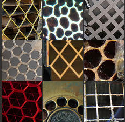
\includegraphics{images/layer-3}
			}
			\subfigure[Activations.]{
				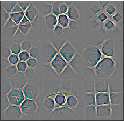
\includegraphics{images/layer-3-activations}
			}
			\caption{Activations of \textbf{layer 3} backprojected to pixel level \cite{ZeilerFergus:2013}.}
		\end{figure}
	\end{frame}
	
	\begin{frame}{Feature Activations (cont'd)}
		\begin{figure}
			\centering
			\subfigure[Images.]{
				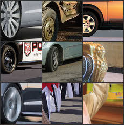
\includegraphics{images/layer-3-2}
			}
			\subfigure[Activations.]{
				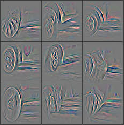
\includegraphics{images/layer-3-activations-2}
			}
			\caption{Activations of \textbf{layer 3} backprojected to pixel level \cite{ZeilerFergus:2013}.}
		\end{figure}
	\end{frame}
	
	\begin{frame}{Feature Activations (cont'd)}
		\begin{figure}
			\centering
			\subfigure[Images.]{
				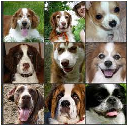
\includegraphics{images/layer-4}
			}
			\subfigure[Activations.]{
				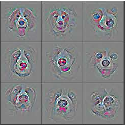
\includegraphics{images/layer-4-activations}
			}
			\caption{Activations of \textbf{layer 4} backprojected to pixel level \cite{ZeilerFergus:2013}.}
		\end{figure}
	\end{frame}
	
	\begin{frame}{Feature Activations (cont'd)}
		\begin{figure}
			\centering
			\subfigure[Images.]{
				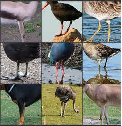
\includegraphics{images/layer-4-2}
			}
			\subfigure[Activations.]{
				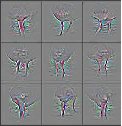
\includegraphics{images/layer-4-activations-2}
			}
			\caption{Activations of \textbf{layer 4} backprojected to pixel level \cite{ZeilerFergus:2013}.}
		\end{figure}
	\end{frame}
	
	\section{Conclusion}
	\begin{frame}{Conclusion}
		Convolutional networks perform well in computer vision tasks as they learn a feature hierarchy.
		\vskip 1em
		
		Internal workings of convolutional networks are not well understood.
		\vskip 1em
		
		\begin{itemize}
			\item \cite{ZeilerFergus:2013} use \textit{de}convolutional networks to visualize feature activations;
			\item this allows to analyze the feature hierarchy and to increase performance.
			\begin{itemize}
				\item For example by adjusting the filter size and subsampling scheme.
			\end{itemize}
		\end{itemize}
	\end{frame}
	
	\begin{frame}{The End}
		\begin{center}
			{\LARGE Thanks for your attention!}
			\vskip .25em
			Paper available at \url{http://davidstutz.de/seminar-paper-understanding-convolutional-neural-networks/}
			\vskip .25em
			
			\begin{figure}
				\centering
				\subfigure{
					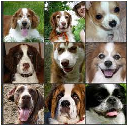
\includegraphics{images/layer-4}
				}
				\subfigure{
					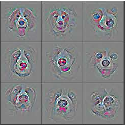
\includegraphics{images/layer-4-activations}
				}
			\end{figure}
			\vskip .5em
			
			{\Large Questions?}
		\end{center}
	\end{frame}
	
	\bibliographystyle{alpha}
	\bibliography{slides}
\end{document}